\documentclass[twoside,10pt]{article}
\usepackage{amsmath,amsfonts,amsthm,fullpage,amssymb}
%\usepackage{mymath}
\usepackage{algorithm}
\usepackage{algorithmic}
\usepackage{graphicx}
\usepackage{url}
\usepackage{listings}
\usepackage{caption}
\usepackage{subcaption}

\begin{document}

\title{ISYE 6740 Homework 4\\ 
\small Total 100 points. 30 points Bonus questions.}
%\author{Yao Xie}
%\date{Deadline: Feb. 13, Sat., 11:55pm}
\date{}
\maketitle

%----------------------------------------------------------------------------------

\begin{enumerate}

\item {\bf Basic optimization.} (50 points.)

The background of logistic regression will be discussed in the next lecture. Here, we just focus on finding out the property of the optimization problem, related to training a logistic regression. 

Consider a simplified logistic regression problem. 
Given $n$ training samples $(x_i, y_i)$, $i = 1, \ldots, n$. The data $x_i \in \mathbb R$, and $y_i \in \{0, 1\}$.  To train/fit a logistic regression model for classification, we solve the following optimization problem, where $\theta \in \mathbb R$ is a parameter we aim to find:
\begin{equation}
\max_\theta \ell (\theta), \label{eqn}
\end{equation}
where the log-likelhood function \[\ell(\theta) = \sum_{i=1}^n \left\{-\log (1+\exp\{-\theta x_i\}) + (y_i-1) \theta x_i\right\}.\]

\begin{enumerate}
\item (15 points) 

Logistic regression model:
$$p(y =1|x,\theta) = \frac{1}{1+\exp(-\theta^Tx)}$$

Note that:
$$p(y =0 |x,\theta) = 1 - \frac{1}{1+\exp(-\theta^Tx)}=\frac{\exp(-\theta^Tx)}{1+\exp(-\theta^Tx)}$$

We are using maximum likelihood so plug in:

$$\max_\theta \ell (\theta):=log \prod_{i=1}^{m}P(y^i|x^i,\theta)$$

$$=\sum(y^i-1)\theta^Tx^i-log(1+\exp(-\theta^Tx^i))$$ 

This is an unconstrined optimization problem, solvable using gradient descent.

\begin{lstlisting}
theta_t = inf
theta_t_1 = rand
error = .01
while abs(theta_t - theta_t_1) > error:
	theta_t = theta_t_1
	theta_t_1 = get_negative_gradient(theta_t_1)
\end{lstlisting}




\item (15 points) {\bf stochastic gradient descent}
For huge datasets it may not be feasible to use gradient descent.  Batch gradient descent can be used to overcome this obstacle by randomly selecting a subset of data and applying gradient descent and eventually looping through all of the data.  The gradient is unbiased so the expectation equals the true gradient.

$$\nabla \hat{\ell} (\theta)=\sum_{y^i\epsilon S_k}(y^i-1)x^i+\frac{\exp(-\theta^Tx^i)x^i}{1+\exp(-\theta^Tx^i)}$$
 
\item (20 points) If a function $f$ is differentiable it can be chatacterized as concave if the negative of the function (that is if $f$ is concave $-f$ is convex) follows the first and second order conditions resulting in a positive semi-definite Hessian.

First order condition:

$$f(y) \geq f(x) + \nabla f(x) ^T (y-x)$$
for all $x,y \epsilon {\rm dom} f$

Second Order condition:
$f$ is convex iff $ {\rm dom} f$ is convex and for all $x \epsilon {\rm dom} f$
$$\nabla^2 f(x) \geq 0$$

  
Solution:

$$l(\theta) = \sum_{i=1}^n \{ -log\left( 1 + e^{-\theta x_i} \right) + \left( y_i - 1 \right)\theta x_i \}$$

$$\begin{bmatrix}
 \frac{\partial^2 l}{\partial \theta_1^2} & \dots & \frac{\partial^2 l}{\partial \theta_1 \partial \theta_n} \\
 \vdots & \ddots & \vdots \\
 \frac{\partial^2 l}{\partial \theta_n \partial \theta_1} & \dots & \frac{\partial^2 l}{\partial \theta_ n^2} \\
\end{bmatrix}
$$

$$
\begin{bmatrix}
\frac{\partial^2 l}{\partial \theta^2} \\
\end{bmatrix}
=-\frac{x^2 \exp(x \theta)}{(\exp(x \theta)+1)^2}
$$

Since we see that the above is indeed a concave function we know that there is a single global maximum and is a great candidate for gradient descent.  Gradient descent travels along the function's gradient in pre defined learning steps until it reaches the maximum.  Since we know that there are not any local maxima once the maximum is found training is complete.

\end{enumerate}
 
\item {\bf Comparing Bayes, logistic, and KNN classifiers.} (50 points)

In lectures we learn three different classifiers. This question is to implement and compare them. We are suggest use \textsf{Scikit-learn}, which is a commonly-used and powerful \textsf{Python} library with various machine learning tools. But you can also use other similar library in other languages of your choice to perform the tasks. 



\textbf{Part One (Divorce classification/prediction).} (30 points) 





Build three classifiers using (Naive Bayes, Logistic Regression, KNN). Use the first $80\%$ data for training and the remaining $20\%$ for testing. If you use \textsf{scikit-learn} you can use \textsf{train\_test\_split} to split the dataset. 

\begin{enumerate}

	\item Report testing accuracy for each of the three classifiers.  Comment on their performance: which performs the best and make a guess why they perform the best in this setting. 
	
Table 1: Accuracy comparison between 3 different classification algorithms.
 
\begin{table}[h!]
\centering
\begin{tabular}{|| c | c | c | c ||} 
 \hline
  & Naive Bayes & Logistic Regression & KNN  \\ [0.5ex] 
 \hline\hline
 Accuracy & .971 & .971 & .971 \\ 
 \hline
\end{tabular}
\label{table:1}
\end{table}

All classification algorithms performed equally against the divorce dataset with an accuracy of 97.1\% seen in table 1 above.  I am surprised that logistic regression and naive bayes performed equally because of the different modeling assumptions associated with each.  Although both algorithms are paramtetric models Naive Bayes assumes all features to be independent of each other, where logistic regression does not.  I would expect the features of divorce to be correlated and the two algorithms to perform differently.

KNN is a non-parametric model that labels any new data by selecting k nearest neighbors and labeling it with the majority label of those neighbors.  Looking at the decision boundary the data seems to be easily separated with very few datapoints crossing the decision boundary.  This seems like a well suited task for KNN.



	\item Use the first two features to train three new classifiers. Plot the data points and decision boundary of each classifier. Comment on the difference between the decision boundary for the three classifiers. Please clearly represent the data points with different labels using different colors.
\end{enumerate}


\begin{figure}[h]
  \begin{subfigure}[b]{0.3\textwidth}
    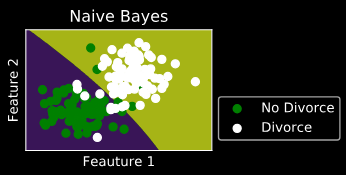
\includegraphics[width=\textwidth]{nb.png}
    \caption{Naive Bayes.}
    \label{fig:f1}
  \end{subfigure}
  \hfill
  \begin{subfigure}[b]{0.3\textwidth}
    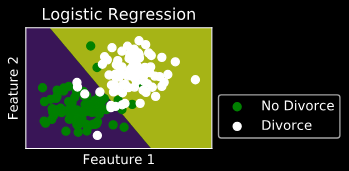
\includegraphics[width=\textwidth]{lr.png}
    \caption{Logistic Regression.}
    \label{fig:f2}
  \end{subfigure}
  \hfill
  \begin{subfigure}[b]{0.3\textwidth}
    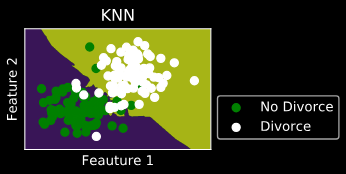
\includegraphics[width=\textwidth]{knn.png}
    \caption{KNN.}
    \label{fig:f3}
  \end{subfigure}
  \caption{Decision Boundaries for 3 classification algorithms.}
\end{figure}


\textbf{Part Two (Handwritten digits classification).} (20 points) Repeat the above using the \textbf{MNIST Data} in our \textbf{Homework 3}. Here, give ``digit'' 6 label $y = 1$, and give ``digit'' 2 label $y = 0$. All the pixels in each image will be the feature (predictor variables) for that sample (i.e., image). Our goal is to build classifier to such that given a new test sample, we can tell is it a 2 or a 6. Using the first $80\%$ of the samples for training and remaining $20\%$ for testing. Report the classification accuracy on testing data, for each of the three classifiers. Comment on their performance: which performs the best and make a guess why they perform the best in this setting.



\begin{table}[h!]
\centering
\begin{tabular}{|| c | c | c | c ||} 
 \hline
  & Naive Bayes & Logistic Regression & KNN  \\ [0.5ex] 
 \hline\hline
 Accuracy & .807 & .982 & .997 \\ 
 \hline
\end{tabular}
\label{table:2}
\end{table}


Naive Bayes performed the worst of the three algorithms at 80.7\% accuracy.  Making the assumption that all features are independent of each other on such a large feature space as images often are was probably what led to such a poor performance.  

Logistic Regression did much better with 98.2\% accuracy.  The 2 and the 6 are very different looking digits which allows logistic regression to make a linear separation of the 2.

KNN outperformed Naive Bayes and logisitic regression.  For the same reason that logistic regression did well, the 2 and 6 are quite different looking values from each other and using distance as a metric is probably a good one in this instance.  I would not expect this performance if the data consisted of 2 similar looking digits such as 1 and 7 for example. 









\end{enumerate}


\end{document}
